\documentclass[12pt]{article}

\usepackage[top=1in, bottom=1in, left=1in, right=1in]{geometry} 
\usepackage{graphicx}
\usepackage{setspace}
\usepackage{bm}
\usepackage{amsmath}
\usepackage{amssymb,amsmath}
\usepackage{listings}
\usepackage{color}
\usepackage{enumitem}
\usepackage{fancyvrb}
\usepackage{hyperref}
\usepackage{diagbox}
\usepackage{float}
\geometry{letterpaper}
\linespread{1.1}% \geometry{landscape} % rotated page geometry

\definecolor{codegreen}{rgb}{0,0.6,0}
\definecolor{codegray}{rgb}{0.5,0.5,0.5}
\definecolor{codepurple}{rgb}{0.58,0,0.82}
\definecolor{backcolour}{rgb}{0.95,0.95,0.92}
\definecolor{outcolor}{rgb}{0.545, 0.0, 0.0}

\lstdefinestyle{mystyle}{
	backgroundcolor=\color{backcolour},   
	commentstyle=\color{codegreen},
	keywordstyle=\color{magenta},
	numberstyle=\tiny\color{codegray},
	stringstyle=\color{codepurple},
	basicstyle=\footnotesize,
	breakatwhitespace=false,         
	breaklines=true,                 
	captionpos=b,                    
	keepspaces=true,                 
	numbers=left,                    
	numbersep=5pt,                  
	showspaces=false,                
	showstringspaces=false,
	showtabs=false,                  
	tabsize=2
}

\lstset{style=mystyle}

\title{HW 2: State Estimation in Oil \& Gas Well Drilling}
\date{16 Feb. 2018} 
\author{Franklin Zhao \\ SID: 3033030808}

\begin{document}
	
	\maketitle
	\newcommand{\tabitem}{~~\llap{\textbullet}~~}
	\renewcommand\theequation{\arabic{equation}}
	\renewcommand{\figurename}{Fig.}
	\renewcommand\thesection{Problem \arabic{section}:}
	\renewcommand\thesubsection{(\alph{subsection})}
	\onehalfspacing
	
\section{Dynamic System Modeling}
\subsection{}
\textbf{Modeling objective:} The objective is to formulate a mathmetical model that estimates the drill bit velocity given the table torque $T(t)$.\\
\textbf{Controllable input:} Table torque $\bf{T(t)}$\\
\textbf{Uncontrollable input:} Frictional torque $\bf{T_f(t)}$\\
\textbf{Measured output:} Table velocity $\bf{\omega_T(t)}$\\
\textbf{Performance output:} Bit velocity $\bf{\omega_B(t)}$
\subsection{}
For the top/table:
\begin{equation}
J_T\ddot{\theta}_T(t)=-k(\theta_T(t)-\theta_B(t))-b\omega_T(t)+T(t)
\end{equation}
For the bottom/bit:
\begin{equation}
J_B\ddot{\theta}_B(t)=k(\theta_T(t)-\theta_B(t))-b\omega_B(t)-T_f(t)
\end{equation}
\subsection{}
\begin{equation}
\frac{\partial}{\partial t}\left[
\begin{array}{c}
\theta_T\\
\dot\theta_T\\
\theta_B\\
\dot\theta_B
\end{array}\right]=\underbrace{\left[
\begin{array}{cccc}
0&1&0&0\\
-\frac{k}{J_T}&-\frac{b}{J_T}&\frac{k}{J_T}&0\\
0&0&0&1\\
\frac{k}{J_B}&0&-\frac{k}{J_B}&-\frac{b}{J_B}
\end{array}\right]}_\text{\textbf{A}}\left[
\begin{array}{c}
\theta_T\\
\dot\theta_T\\
\theta_B\\
\dot\theta_B
\end{array}\right]+\underbrace{\left[
\begin{array}{c}
0\\
\frac{1}{J_T}\\
0\\
0
\end{array}
\right]}_\text{\textbf{B}}T+\left[
\begin{array}{c}
0\\
0\\
0\\
-\frac{1}{J_B}
\end{array}
\right]T_f
\end{equation}
\begin{equation}
\dot\theta_T=\underbrace{\left[
\begin{array}{cccc}
0&1&0&0
\end{array}
\right]}_\text{\textbf{C}}\left[
\begin{array}{c}
\theta_T\\
\dot\theta_T\\
\theta_B\\
\dot\theta_B
\end{array}
\right]
\end{equation}
\section{Observability Analysis}
\subsection{}
\lstinputlisting[language=Python]{2a.py}
\begin{Verbatim}
Rank of Observability Matrix for four-state system: 3
\end{Verbatim}
Since $rank(\mathcal{O})=3<4$, $(A,C)$ is not observable.
\subsection{}
\begin{equation}
\frac{\partial}{\partial t}\left[
\begin{array}{c}
\theta\\
\dot\theta_T\\
\dot\theta_B
\end{array}\right]=\underbrace{\left[
	\begin{array}{ccc}
	0&1&-1\\
	-\frac{k}{J_t}&-\frac{b}{J_t}&0\\
	\frac{k}{J_B}&0&-\frac{b}{J_B}
	\end{array}\right]}_\text{\textbf{A}}\left[
\begin{array}{c}
\theta\\
\dot\theta_T\\
\dot\theta_B
\end{array}\right]+\underbrace{\left[
	\begin{array}{c}
	0\\
	\frac{1}{J_T}\\
	0
	\end{array}
	\right]}_\text{\textbf{B}}T+\left[
\begin{array}{c}
0\\
0\\
-\frac{1}{J_B}
\end{array}
\right]T_f
\end{equation}
\begin{equation}
\dot\theta_T=\underbrace{\left[
	\begin{array}{cccc}
	0&1&0
	\end{array}
	\right]}_\text{\textbf{C}}\left[
\begin{array}{c}
\theta\\
\dot\theta_T\\
\dot\theta_B
\end{array}
\right]
\end{equation}
\subsection{}
\lstinputlisting[language=Python]{2c.py}
\begin{Verbatim}
Rank of Observability Matrix for three-state system: 3
\end{Verbatim}
Since $rank(\mathcal{O})=3$, $(A,C)$ is observable.
\section{Measurement Data}
\lstinputlisting[language=Python]{3.py}
The plots of table torque and measured table velocity versus time are shown in Figure~\ref{fig:3}.
\begin{figure}[H]
	\centering
	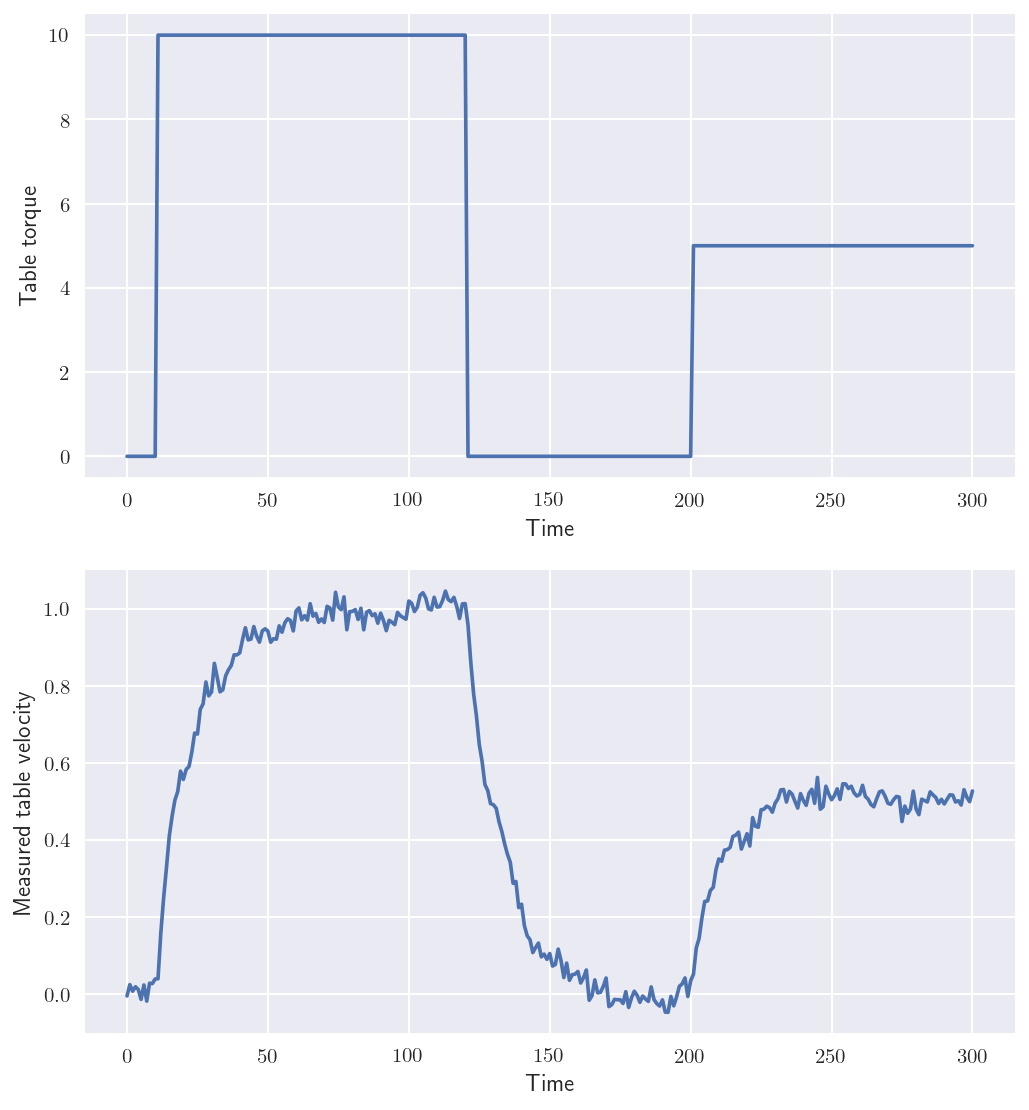
\includegraphics[width=\linewidth]{3.png}      
	\caption{Table torque and measured table velocity versus time}
	\label{fig:3}
\end{figure}
\section{Luenberger Observer}
\subsection{}
Denote $\left[
\begin{array}{c}
\hat\theta\\
\hat{\dot\theta}_T\\
\hat{\dot\theta}_B
\end{array}
\right]$ by $\hat x(t)$, $\hat{\dot\theta}_T$ by $\hat y(t)$, $T(t)$ by $u(t)$, and the Luenberger observer equations will be:
\begin{equation}\label{eq:luen1}
\dot{\hat x}(t)=A\hat x(t)+Bu(t)+L[y(t)-\hat y(t)],\ \ \ \hat x(0)=\hat{x}_0
\end{equation}
\begin{equation}\label{eq:luen2}
\hat y(t)=C\hat x(t)
\end{equation}
\lstinputlisting[language=Python]{4a.py}
\begin{Verbatim}
Eigenvalues of open-loop system: 
[-0.08338525+0.29860789j -0.08338525-0.29860789j -0.08322949+0.j        ]
\end{Verbatim}
\subsection{}
The eigenvalues I chose were $2.5\lambda(A)$. The choice was justified in the RMSE error to be computed and converge speed to be shown in part (d). Basically I chose \{5, 1, 2, 3, 2.5\} and did the validation. It turned out that $2.5\lambda(A)$ was the best choice.
\lstinputlisting[language=Python]{4b.py}
\begin{Verbatim}
L:
[[-25.125]
[  0.375]
[ -0.675]]
\end{Verbatim}
\subsection{}
Write Equation~(\ref{eq:luen1})(\ref{eq:luen2}) in LTI form, and we obtain $A_{lobs}$, $B_{lobs}$, $C_{lobs}$:
\begin{equation}
\dot{\hat x}(t)=\underbrace{(A-LC)}_{A_{lobs}}\hat x(t)+\underbrace{\left[
\begin{array}{cc}
B&L
\end{array}
\right]}_{B_{lobs}}\left[
\begin{array}{c}
u(t)\\
y(t)
\end{array}
\right]
\end{equation}
\begin{equation}
\hat y(t)=C_{lobs}\hat x(t)
\end{equation}
\subsection{}
The eigenvalues I chose were $2.5\lambda(A)$:
\begin{Verbatim}
array([-0.20846314+0.74651974j, -0.20846314-0.74651974j, -0.20807373+0.j])
\end{Verbatim}
\lstinputlisting[language=Python]{4d.py}
\begin{Verbatim}
Luenberger Observer RMSE: 0.0991557694635
\end{Verbatim}
The result of Luenberger observer is shown in Figure~\ref{fig:4}
\begin{figure}[H]
	\centering
	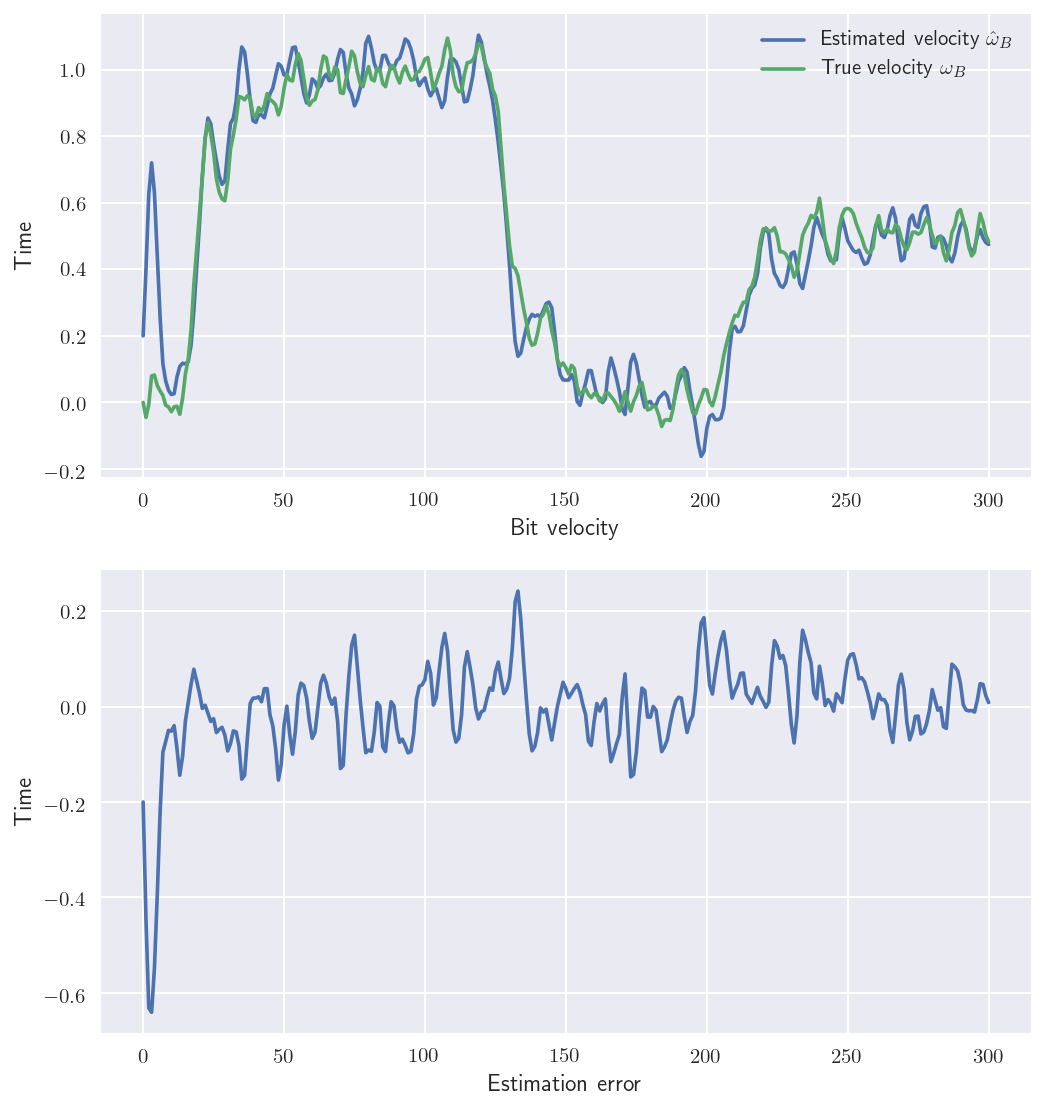
\includegraphics[width=\linewidth]{4.png}      
	\caption{Luenberger observer result}
	\label{fig:4}
\end{figure}
\newpage
\section{Kalman Filter (KF) Design}
\subsection{}
\begin{equation}
\dot{\hat x}(t)=A\hat x(t)+Bu(t)+L(t)(y(t)-\hat y(t))
\end{equation}
\begin{equation}
\hat y(t)=C\hat x(t)
\end{equation}
\begin{equation}
L(t)=\Sigma(t)C^TN^{-1}
\end{equation}
where $\Sigma(t)$ is the solution of the following differential equation:
\begin{equation}
\dot\Sigma(t)=\Sigma(t)A^T+A\Sigma(t)+W-\Sigma(t)C^TN^{-1}C\Sigma(t),\ \ \ \Sigma(0)=\Sigma_0
\end{equation}
where $W$ and $N$ are covariance matrices of $w(t)$ and $n(t)$.
\subsection{}
\lstinputlisting[language=Python]{5b.py}
\begin{Verbatim}
Kalman Filter RMSE: 0.0560275348234 rad/s
\end{Verbatim}
The value of $W$ I tuned is listed as follow. Basically I determined the magnitude first. Then based on the plots in part (c), I tuned the diagonal elements, and finally tuned other elements. It turned out that the RMSE did not change too much, but $\Sigma_{33}$ changed dramatically. 
\begin{Verbatim}
W = np.matrix([[0.0006, 0.005, 0.001], 
	       [0.02,   0.003, 0.004], 
	       [0.004,  0.001, 0.003]])
\end{Verbatim}
\subsection{}
\lstinputlisting[language=Python]{5c.py}
The result of Kalman Filter is shown in Figure~\ref{fig:5}.
\begin{figure}[H]
	\centering
	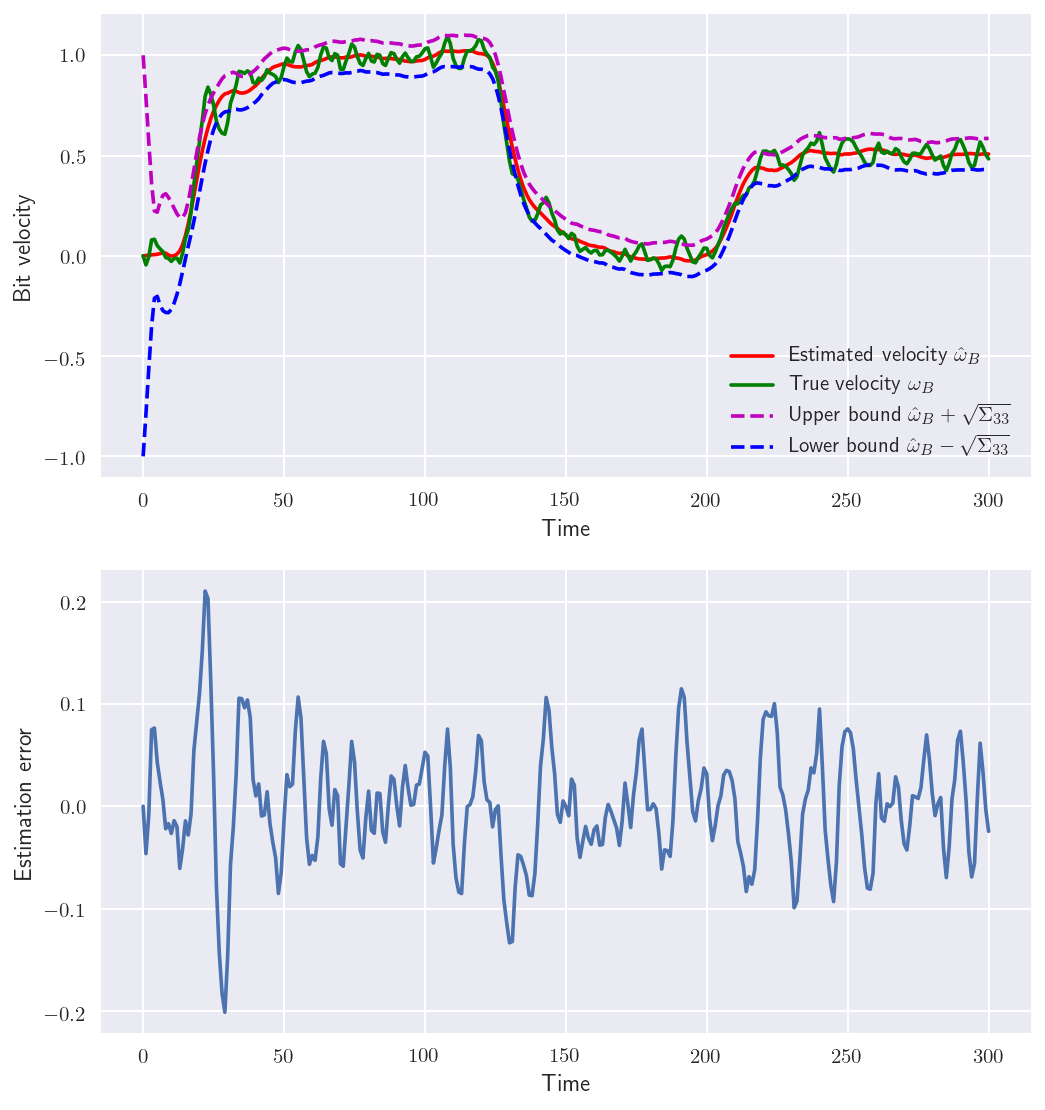
\includegraphics[width=\linewidth]{5.png}      
	\caption{Kalman filter result}
	\label{fig:5}
\end{figure}
\subsection{}
\lstinputlisting[language=Python]{5d.py}
\begin{Verbatim}
array([-0.08707987+0.2849352j, -0.08707987-0.2849352j, -0.34475403+0.j])
\end{Verbatim}
The 1st and 2nd poles are very close to the eigenvalues I chose in the Luenberger observer, but the 3rd one is a bit more different.
\section{Extended Kalman Filter (EKF) Design}
Replace Hooke's law with nonlinear spring torque relationship, and the EKF can be obtained:
\begin{equation}
\underbrace{\frac{\partial}{\partial t}\left[
\begin{array}{c}
\theta\\
\dot\theta_T\\
\dot\theta_B
\end{array}
\right]}_{\hat x(t)}=\underbrace{\left[
\begin{array}{c}
\hat\theta_T - \hat\theta_B\\
\frac{-k_1\theta-k_2\theta^3-b\dot\theta_T+T(t)}{J_T}\\
\frac{k_1\theta+k_2\theta^3-b\dot\theta_B}{J_B}
\end{array}	
\right]}_{f(x(t),u(t))}+w(t),\ \ \ x(0)=x_0
\end{equation} 
\begin{equation}
\dot\theta_T=\underbrace{C\left[
\begin{array}{c}
\theta\\
\dot\theta_T\\
\dot\theta_B
\end{array}
\right]}_{h(x(t),u(t))}+n(t)
\end{equation}
Hence, $F(t)$ and $H(t)$ can be derived:
\begin{equation}
F(t)=\frac{\partial f}{\partial x}(\hat x(t),u(t))=\left[
\begin{array}{ccc}
0&1&-1\\
\frac{-k_1-3k_2\hat\theta^2}{J_T}&\frac{-b}{J_T}&0\\
\frac{k_1+3k_2\hat\theta^2}{J_B}&0&\frac{-b}{J_B}
\end{array}
\right]
\end{equation}
\begin{equation}
H(t)=\frac{\partial h}{\partial x}(\hat x(t),u(t))=C=\left[
\begin{array}{ccc}
0&1&0
\end{array}\right]
\end{equation}
\lstinputlisting[language=Python]{6.py}
\begin{Verbatim}
Extended Kalman Filter RMSE: 0.0458628285791 rad/s
\end{Verbatim}
The result of EKF is shown in Figure~\ref{fig:6}.
\begin{figure}[H]
	\centering
	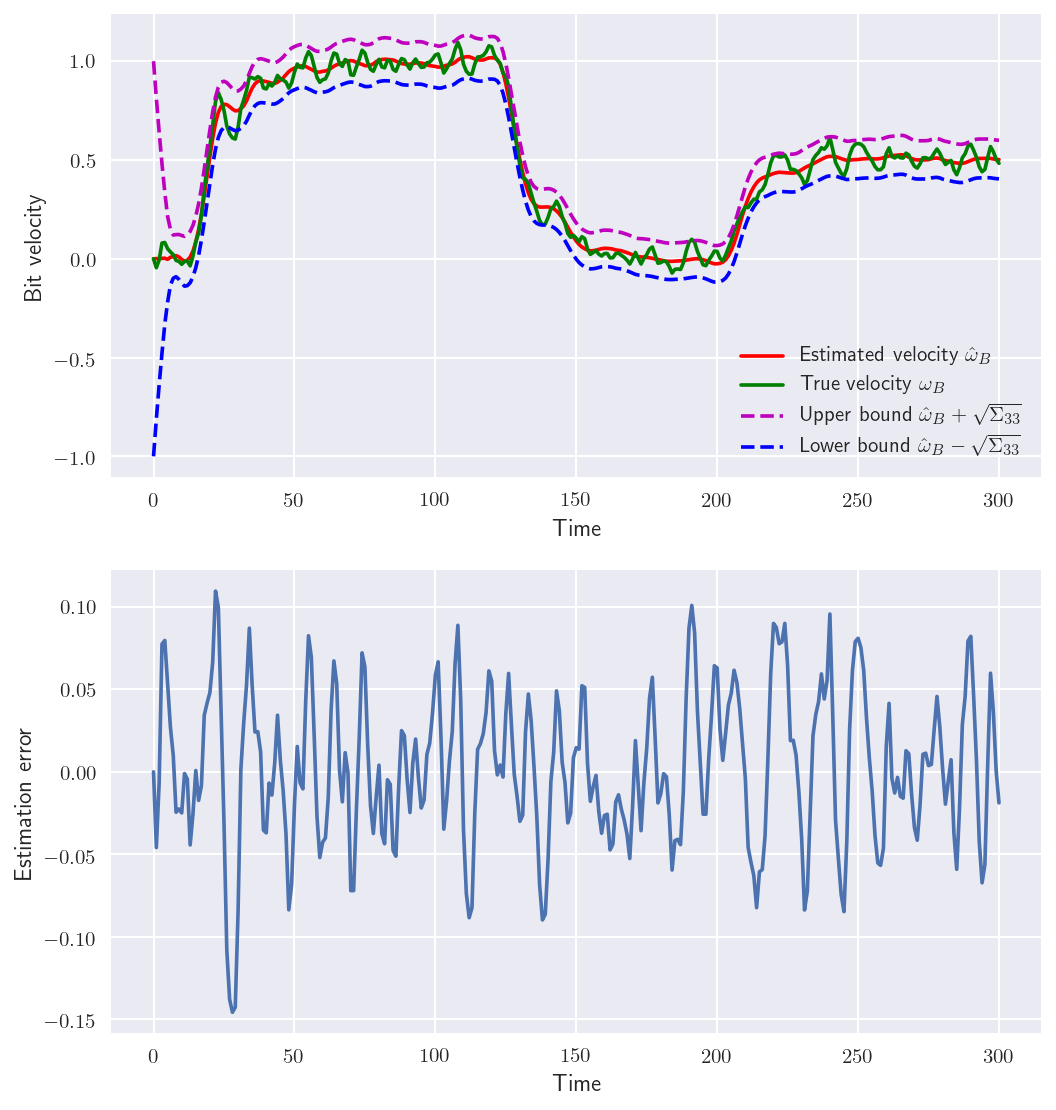
\includegraphics[width=\linewidth]{6.png}      
	\caption{EKF result}
	\label{fig:6}
\end{figure}
\end{document}